\section{Wstęp}

\subsection{Opis problemu}

Głównym założeniem projektu było zapoznanie się biblioteką OpenMP na podstawie równoległego sumowania komórek tablicy. W ramach projektu zrealizowaliśmy 4 algorytmy sekwencyjne oraz 2 algorytmy zrównleglone. Celem zastosowania czterech różnych algorytmów sekwencyjnych było zbadanie wpływu sekcyjności pamięci podręcznej, wyprzdzającego pobrania danych do pamięcy podręcznej oraz kolejności uszeregowania pętli na czas realizacji zadania. W przypadku algorytmów zrównoleglonych badaliśmy wpływ kolejności uszeregowania pętli na końcowy rezultat.\newline

Nasze badania podzieliliśmy na 3 spójne części. Kolejno badaliśmy
\begin{itemize}
\item rozmiar danych
\item sekcyjność pamięci
\item wyprzedzające pobranie
\end{itemize}
na czas realizacji problemu.\newline

Sam problem sprowadzał się do zsumowania wartości komórek w tabeli. Dla zachowania czytelności w kolejności pętli zastosowaliśmy tablicę dwuwymiarową. Ponieważ sam problem jest prosty obliczeniowo zmuszeni byliśmy do stosowania maksymalnego rozmiaru tablicy tj $[2^{28} - wierszy]$ na $[2^{4} - kolumn]$.

\subsection{Punkt odniesienia (algorytm sekwencyjny - kolejność ij)}

Punktem odniesienia dla wszystkich algorytmów był podstawowy algorytm sekwencyjny w którym sumowaliśmy elementy tablicy wierszami. Nazywany dalej $sum\_ij$.

\lstinputlisting{./code/sum_ij.cpp}


\subsection{Badane algorytmy}


\subsubsection{Algorytm sekwencyjny - kolejność ji}

Algorytm sekwencyjny ze zmienioną kolejnością pętli (sumujemy kolumnami). Nazywany dalej $sum\_ji$.
\lstinputlisting{./code/sum_ji.cpp}


\subsubsection{Algorytm zrównoleglony - kolejność ij}

Algorytm sumujący wierszami realizowany równolegle. Nazywany dalej $sum\_par\_ij$.
\lstinputlisting{./code/sum_par_ij.cpp}


\subsubsection{Algorytm zrównoleglony - kolejność jj}

Algorytm realizowany równolegle ze zmienioną kolejnością pętli (sumujemy kolumnami). Nazwywany dalej $sum_par\_ji$.
\lstinputlisting{./code/sum_par_ji.cpp}


\subsubsection{Algorytm na sekcyjność pamięci}

Algorytm sekwencyjny w którym badaliśmy wpływ sekcyjności pamięci na czas wykonania zadania. Nazywany dalej $sum\_sec$.
\lstinputlisting{./code/sum_sec.cpp}


\subsubsection{Algorytm na  pobranie  z wyprzedzeniem}

Algorytm sekwencyjny w którym badaliśmy wpływ wyprzedzającego pobrania danych do pamięci podręcznej na czas realizacji zadania. Nazywany dalej $sum\_pf$.
\lstinputlisting{./code/sum_pf.cpp}

\subsection{Maska powinowactwa}

Aby wyeliminować przełączanie wykonywania wątku pomiędzy rdzeniami procesora zastosowaliśmy maski powinowactwa.

\subsubsection{Kod}

\lstinputlisting{./code/mask.cpp}

\subsubsection{Rezultat}

W rezultacie dla przetwarzania równoległego każdy wątek odpowiedzialny za sumowanie realizowany jest na oddzielnym procesorze. Co widoczne jest na poniższych wykresach:

\begin{figure}[H]
\minipage{0.5\textwidth}
  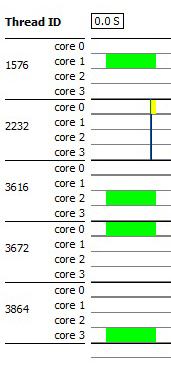
\includegraphics{mask_parallel.png}
  \caption{Wykres wątków dla $sum\_par\_ij$}
\endminipage\hfill
\minipage{0.5\textwidth}
  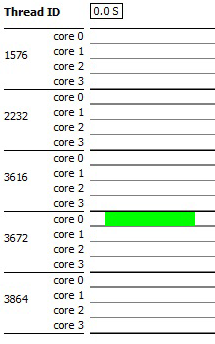
\includegraphics{mask_single.png}
  \caption{Wykres wątków dla $sum\_ij$}
\endminipage\hfill
\end{figure}
